\documentclass[tikz,border=7pt]{standalone}
\begin{document}
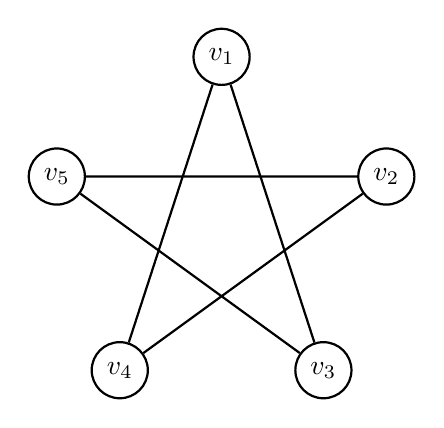
\begin{tikzpicture}[every node/.style={circle,draw,fill=white,minimum size=7mm},line width=.8pt]
\foreach \i/\a in {1/90,2/18,3/-54,4/-126,5/162} \node (v\i) at (\a:2.2) {$v_\i$};
\draw (v1)--(v3) (v1)--(v4) (v2)--(v4) (v2)--(v5) (v3)--(v5);
\end{tikzpicture}
\end{document}
